
\section{Recontrucción}

A la salida del bloque de detección de marcadores se tiene,  para cada cámara y para cada frame de una secuencia adquirida, un conjunto de coordenadas en dos dimensiones x,y que ubican la posición en la imagen de aquellos marcadores que fueron detectados. 
El proceso de reconstrucción consiste en obtener las coordenadas en tres dimensiones de la posición de los marcadores en el espacio a partir de  las coordenadas en dos dimensiones obtenidas en el bloque anterior.
En la figura se muestra un ejemplo de reconstrucción para el caso de dos cámaras.\\


\begin{figure}[h!]
\begin{center}
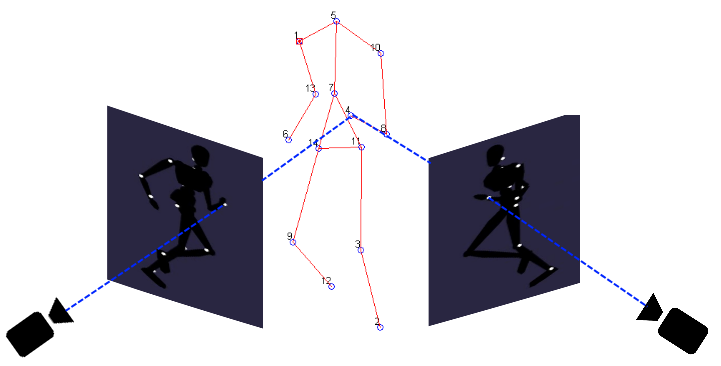
\includegraphics[scale=0.2]{img/Reconstruccion/reconstruccion2.png}
\end{center}
\caption{Reconstruccion con dos camaras}
\label{pinhole_camara}
\end{figure}


Se observa la figura a uno de los marcadores detectados desde las dos vistas y su correspondiente punto 3D reconstruido.\\

El proceso de reconstrucción implementado consiste en dos pasos fundamentales:
\begin{itemize}
\item Determinar  aquellos marcadores detectados en las distintas cámaras que corresponden a un mismo marcador en el espacio. De esta manera se establece una correspondencia entre los marcadores detectados en las distintas vistas.\\
\item Una vez establecidas estas correspondencias se selecciona aquella que con algún criterio pueda se considere más fiable y finalmente se determina las posición en el espacio del marcador.\\

\end{itemize}


\begin{figure}[h!]
\begin{center}
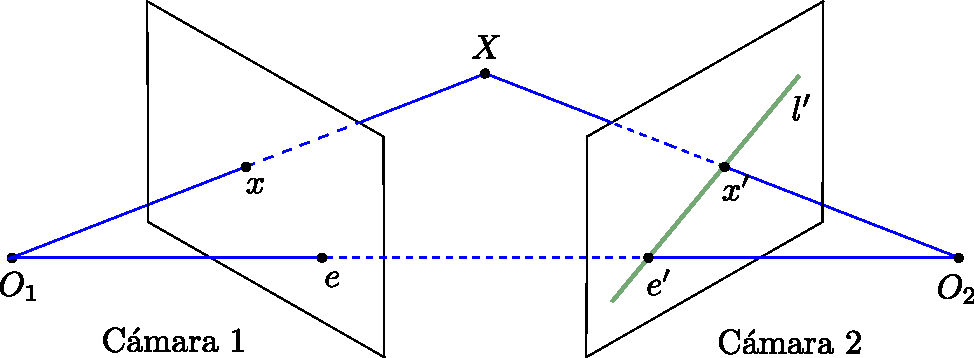
\includegraphics[scale=0.5]{img/Reconstruccion/geometria_epipolar.pdf}
\end{center}
\caption{Reconstruccion con dos camaras}
\label{pinhole_camara}
\end{figure}

Como se explicó anteriormente, se inicia la implementación de este bloque a partir del algoritmo propuesto por herda para este caso. A este algoritmo se le hicieron cambios debido a interpretaciones rellizadas sobre aspectos del algoritmo que no han quedado del todo establecidas y a pruebas que se hicieron luego  para probar su rendimiento.\\

